\section{Hauptteil}
\subsection{Aufgabenbeschreibung und Problemstellung}

In dieser Komplexen Leistung beschreibe ich einen von mir entwickelten Algorithmus zur Lösung der 4. Aufgabe \glqq Krocket\grqq{} des 43. Bundeswettbewerb Informatik. Krocket ist eine Präzisions- und Taktik-Sportart (\hyperref[fig:spieler]{Abb. 1}) in der es das Ziel ist, Bälle durch Tore zu schießen und so zu punkten \cite{krocket_regeln}.


\begin{figure}[h]
\label{fig:spieler}
    \centering
    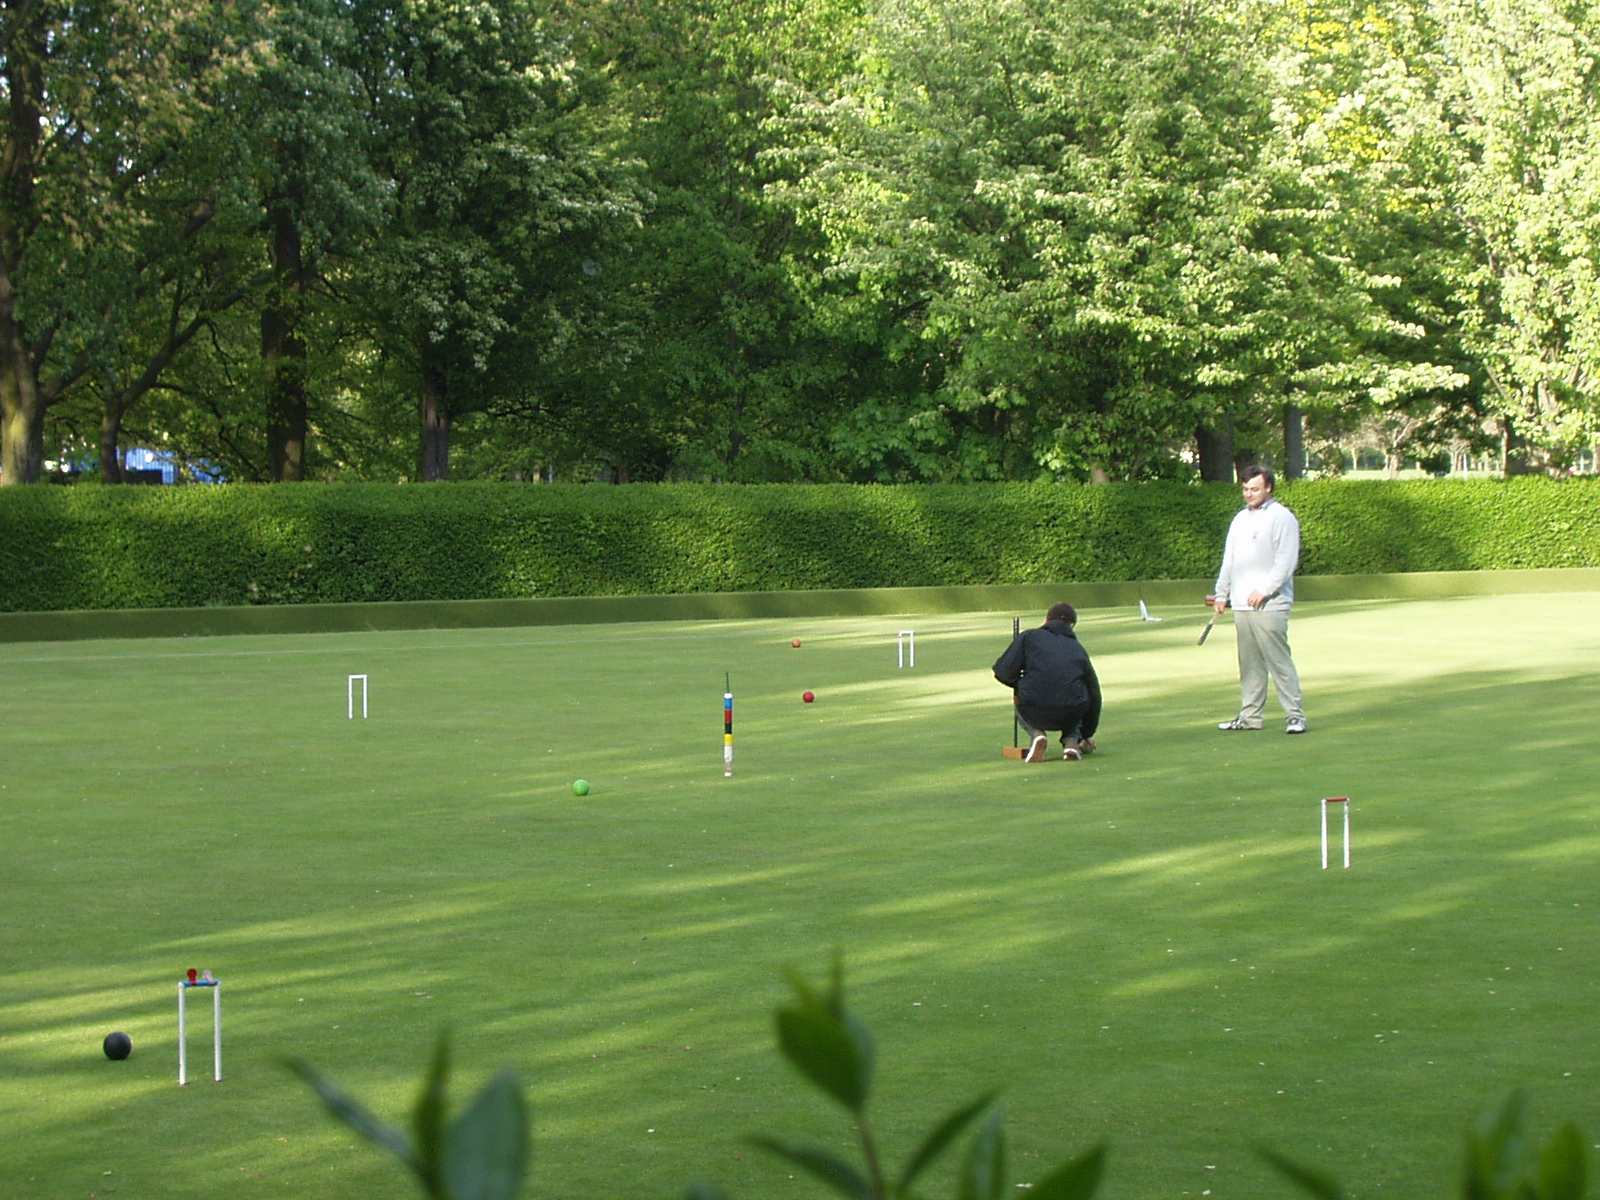
\includegraphics[width=0.8\linewidth]{images/krocketspieler.jpg}
    \caption{Krocketspieler in Edinburgh, Schottland. User:pschemp, CC BY-SA 3.0 <http://creativecommons.org/licenses/by-sa/3.0/>, via Wikimedia Commons}

\end{figure}

Es wird zunächst die Aufgabe beschrieben:

\textbf{Aufgabentext aus der 1. Runde des 43. Bundeswettbewerbs Informatik:}
\begin{quote}
	``Laura findet beim Spielen im Garten einige aufgestellte Tore eines Krocketspiels. Ihr Vater ruft aus der Küche, dass er es mit nur zwei Schlägen geschafft hat, den Ball durch alle Tore in der richtigen Reihenfolge zu stoßen. Das möchte Laura verbessern, wobei sie sich allerdings erlaubt, von einem selbst gewählten Punkt aus abzuschlagen. Aber geht das überhaupt?
	
	Aufgabe 4: Hilf Laura, indem du ein Programm schreibst, das überprüft, ob alle Tore in der richtigen Reihenfolge mit nur einem Schlag durchquert werden können. Falls ja, soll dein Programm ein entsprechendes Paar aus Startpunkt und Schlagrichtung ausgeben. Der Ball ist rund und hat einen in der Eingabe angegebenen Radius $r$. Die Tore sehen von oben wie verschieden lange Geradensegmente aus und sind in der vorgeschriebenen Reihenfolge jeweils durch ihre zwei Endpunkte dargestellt. Hinweis: Es ist hilfreich, den Radius des Balls in einem ersten Lösungsversuch zu vernachlässigen, das heißt $r=0$ anzunehmen.'' \cite{aufgaben}
\end{quote}

Die Lösung der Aufgabe muss also überprüfen, ob es möglich ist, einen Ball mit nur einem einzigen Schlag so zu schießen, dass er alle Tore passiert. Dabei müssen sowohl der Ballradius $r$ als auch die Reihenfolge der Tore beachtet werden. Wenn der Ball alle Tore zwar durchschießen kann, aber nur in der falschen Reihenfolge, ist die Aufgabe nicht lösbar. Die Positionen und Anzahl der Tore sowie der Ballradius sind gegeben. Die Lösung muss eine Gerade $g_1$ zurückgeben. Diese Gerade muss einen Mindestabstand $r$ zu allen Toren haben, damit der Ball auf der Geraden durch alle Tore geschossen werden kann.